\documentclass{standalone}
\usepackage{tikz}
\usetikzlibrary{patterns, positioning}
\usetikzlibrary{shapes.misc}
\usepackage[outline]{contour}
\contourlength{1.5pt} 
\usepackage[sfdefault]{ClearSans} %% option 'sfdefault' activates Clear Sans as the default text font
\usepackage[T1]{fontenc}

\begin{document}
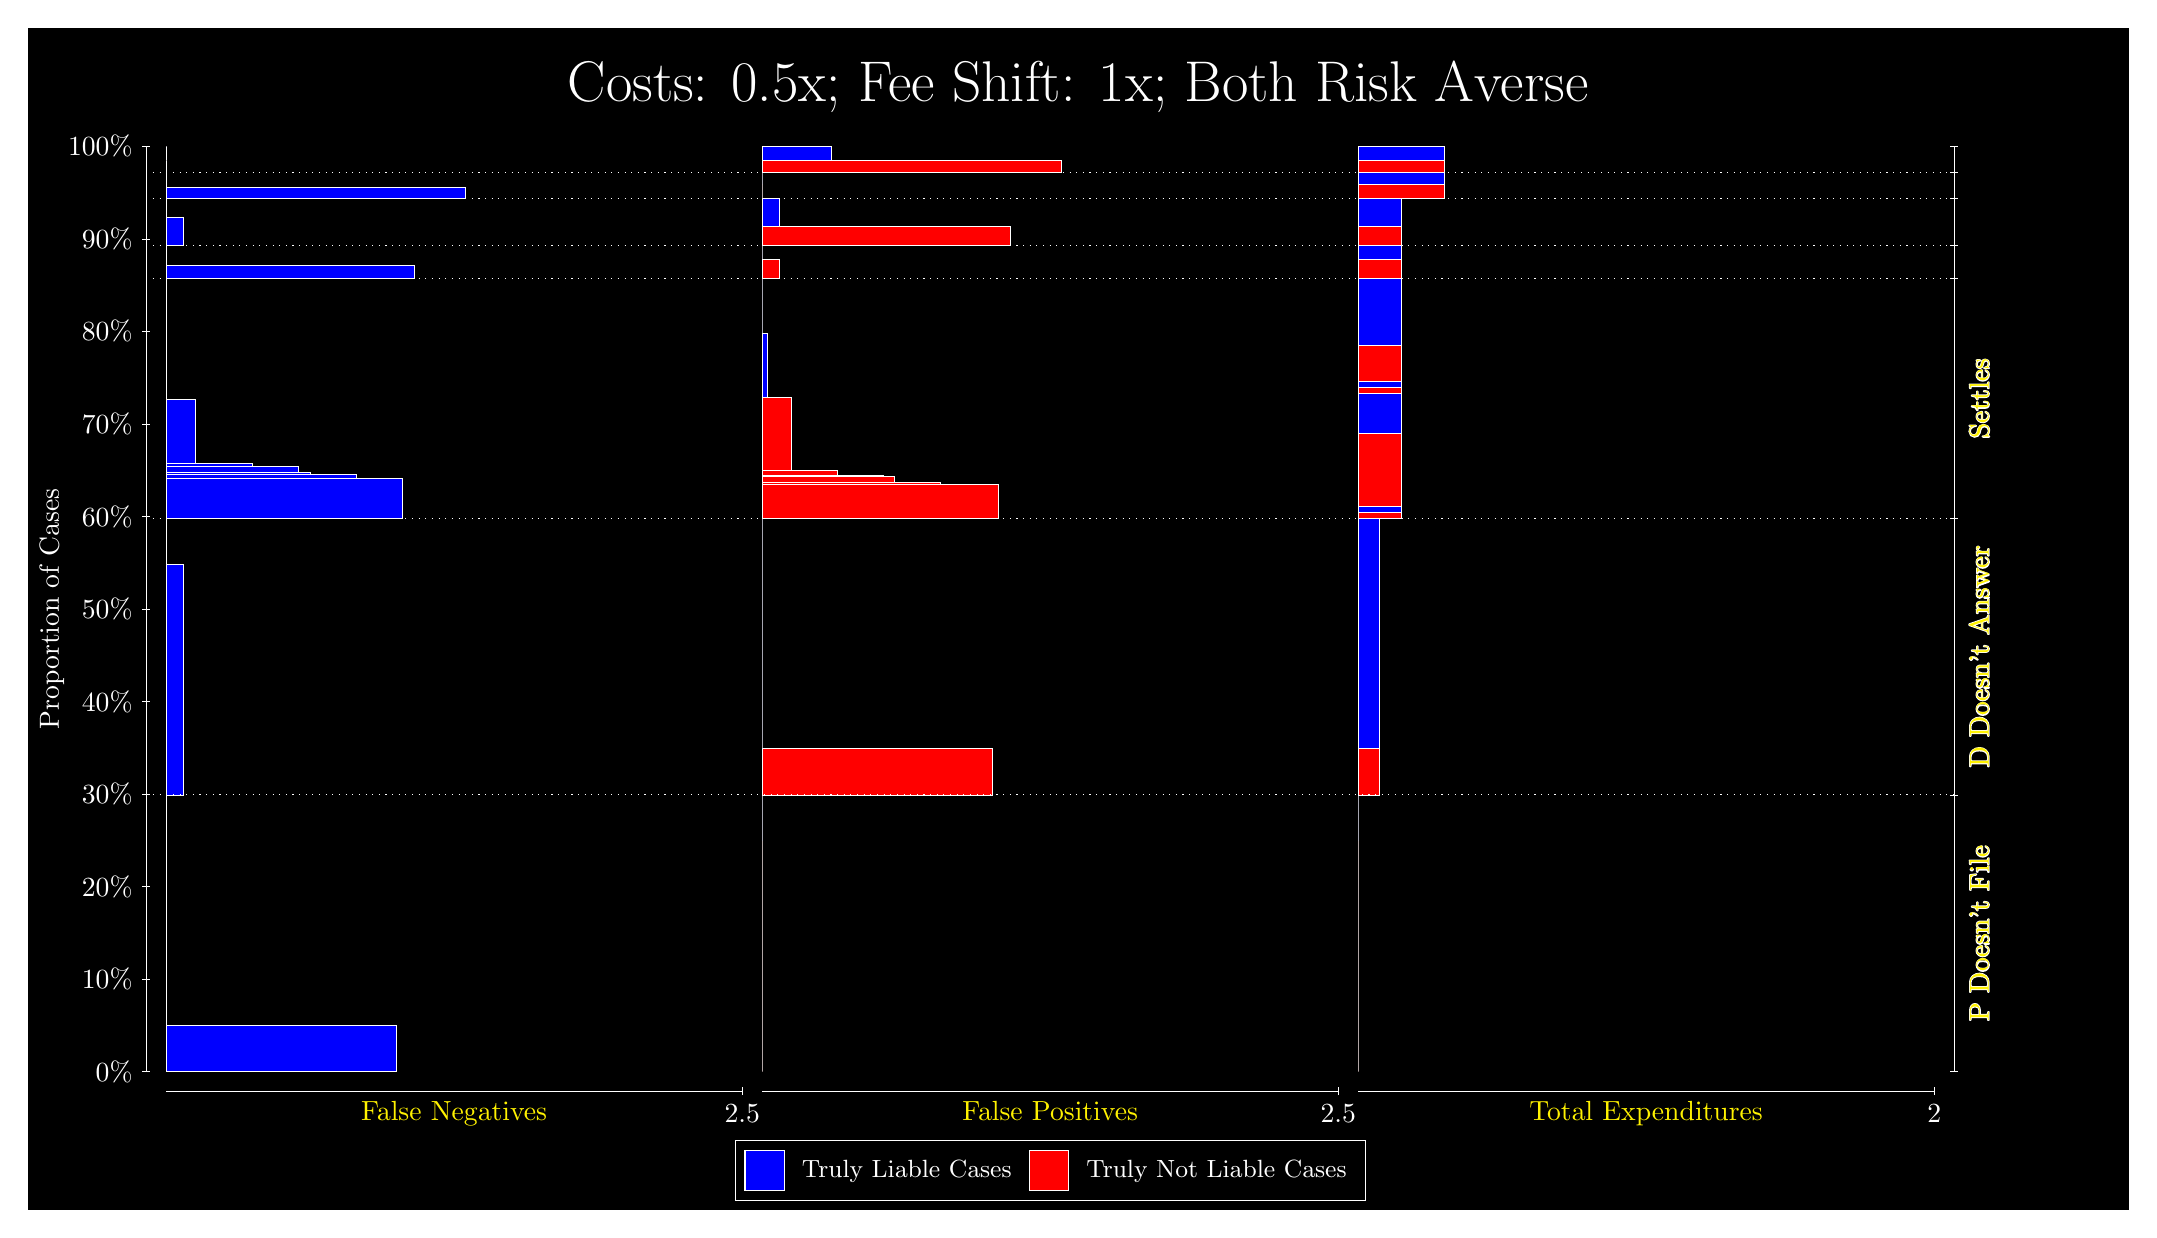
\begin{tikzpicture}
\draw[fill=black] (0,0) rectangle (26.667,15);
\draw[text=white] (0,13.5) rectangle (26.667,15) node[midway] {\huge Costs: 0.5x; Fee Shift: 1x; Both Risk Averse};
\draw[white, very thin] (1.5,1.75) -- (1.5,13.5);
\node[rotate=90, text=white, anchor=center] at (0.3, 7.625) {Proportion of Cases};
\draw[white, very thin] (1.45,1.75) -- (1.55,1.75);
\node[text=white, anchor=east] at (1.45, 1.75) {0\%};
\draw[white, very thin] (1.45,2.925) -- (1.55,2.925);
\node[text=white, anchor=east] at (1.45, 2.925) {10\%};
\draw[white, very thin] (1.45,4.1) -- (1.55,4.1);
\node[text=white, anchor=east] at (1.45, 4.1) {20\%};
\draw[white, very thin] (1.45,5.275) -- (1.55,5.275);
\node[text=white, anchor=east] at (1.45, 5.275) {30\%};
\draw[white, very thin] (1.45,6.45) -- (1.55,6.45);
\node[text=white, anchor=east] at (1.45, 6.45) {40\%};
\draw[white, very thin] (1.45,7.625) -- (1.55,7.625);
\node[text=white, anchor=east] at (1.45, 7.625) {50\%};
\draw[white, very thin] (1.45,8.8) -- (1.55,8.8);
\node[text=white, anchor=east] at (1.45, 8.8) {60\%};
\draw[white, very thin] (1.45,9.975) -- (1.55,9.975);
\node[text=white, anchor=east] at (1.45, 9.975) {70\%};
\draw[white, very thin] (1.45,11.15) -- (1.55,11.15);
\node[text=white, anchor=east] at (1.45, 11.15) {80\%};
\draw[white, very thin] (1.45,12.325) -- (1.55,12.325);
\node[text=white, anchor=east] at (1.45, 12.325) {90\%};
\draw[white, very thin] (1.45,13.5) -- (1.55,13.5);
\node[text=white, anchor=east] at (1.45, 13.5) {100\%};

\draw[white, very thin] (24.457,1.75) -- (24.457,13.5);
\draw[white, very thin] (24.407,1.75) -- (24.507,1.75);
\node[anchor=west] at (24.407, 1.75) {};
\draw[white, very thin] (24.407,5.2642) -- (24.507,5.2642);
\node[anchor=west] at (24.407, 5.2642) {};
\draw[white, very thin] (24.407,8.7774) -- (24.507,8.7774);
\node[anchor=west] at (24.407, 8.7774) {};
\draw[white, very thin] (24.407,11.82) -- (24.507,11.82);
\node[anchor=west] at (24.407, 11.82) {};
\draw[white, very thin] (24.407,12.245) -- (24.507,12.245);
\node[anchor=west] at (24.407, 12.245) {};
\draw[white, very thin] (24.407,12.837) -- (24.507,12.837);
\node[anchor=west] at (24.407, 12.837) {};
\draw[white, very thin] (24.407,13.168) -- (24.507,13.168);
\node[anchor=west] at (24.407, 13.168) {};
\draw[white, very thin] (24.407,13.5) -- (24.507,13.5);
\node[anchor=west] at (24.407, 13.5) {};

\draw[white, very thin, fill=blue] (1.75,1.75) rectangle (4.6775,2.3359);
\draw[white, very thin, fill=red] (1.75,2.3359) rectangle (1.75,5.2642);
\draw[white, very thin, fill=blue] (1.75,5.2642) rectangle (1.9696,8.1921);
\draw[white, very thin, fill=red] (1.75,8.1921) rectangle (1.75,8.7774);
\draw[white, very thin, fill=blue] (1.75,8.7774) rectangle (4.7507,9.2863);
\draw[white, very thin, fill=blue] (1.75,9.2863) rectangle (4.1652,9.3393);
\draw[white, very thin, fill=blue] (1.75,9.3393) rectangle (3.5797,9.3568);
\draw[white, very thin, fill=blue] (1.75,9.3568) rectangle (3.4333,9.4392);
\draw[white, very thin, fill=blue] (1.75,9.4392) rectangle (2.8478,9.4702);
\draw[white, very thin, fill=blue] (1.75,9.4702) rectangle (2.1159,10.283);
\draw[white, very thin, fill=red] (1.75,10.283) rectangle (1.75,11.82);
\draw[white, very thin, fill=blue] (1.75,11.82) rectangle (4.8971,11.995);
\draw[white, very thin, fill=red] (1.75,11.995) rectangle (1.75,12.245);
\draw[white, very thin, fill=blue] (1.75,12.245) rectangle (1.9696,12.594);
\draw[white, very thin, fill=red] (1.75,12.594) rectangle (1.75,12.837);
\draw[white, very thin, fill=blue] (1.75,12.837) rectangle (5.5558,12.986);
\draw[white, very thin, fill=red] (1.75,12.986) rectangle (1.75,13.168);
\draw[white, very thin, fill=red] (1.75,13.168) rectangle (1.75,13.318);
\draw[white, very thin, fill=blue] (1.75,13.318) rectangle (1.75,13.5);
\draw[white, very thin, fill=red] (9.3189,1.75) rectangle (9.3189,4.6783);
\draw[white, very thin, fill=blue] (9.3189,4.6783) rectangle (9.3189,5.2642);
\draw[white, very thin, fill=red] (9.3189,5.2642) rectangle (12.246,5.8495);
\draw[white, very thin, fill=blue] (9.3189,5.8495) rectangle (9.3189,8.7774);
\draw[white, very thin, fill=red] (9.3189,8.7774) rectangle (12.32,9.2039);
\draw[white, very thin, fill=red] (9.3189,9.2039) rectangle (11.588,9.231);
\draw[white, very thin, fill=red] (9.3189,9.231) rectangle (11.002,9.3106);
\draw[white, very thin, fill=red] (9.3189,9.3106) rectangle (10.856,9.3281);
\draw[white, very thin, fill=red] (9.3189,9.3281) rectangle (10.27,9.3869);
\draw[white, very thin, fill=red] (9.3189,9.3869) rectangle (9.6848,10.314);
\draw[white, very thin, fill=blue] (9.3189,10.314) rectangle (9.3921,11.127);
\draw[white, very thin, fill=blue] (9.3189,11.127) rectangle (9.3189,11.82);
\draw[white, very thin, fill=red] (9.3189,11.82) rectangle (9.5384,12.07);
\draw[white, very thin, fill=blue] (9.3189,12.07) rectangle (9.3189,12.245);
\draw[white, very thin, fill=red] (9.3189,12.245) rectangle (12.466,12.488);
\draw[white, very thin, fill=blue] (9.3189,12.488) rectangle (9.5384,12.837);
\draw[white, very thin, fill=red] (9.3189,12.837) rectangle (9.3189,13.019);
\draw[white, very thin, fill=blue] (9.3189,13.019) rectangle (9.3189,13.168);
\draw[white, very thin, fill=red] (9.3189,13.168) rectangle (13.125,13.318);
\draw[white, very thin, fill=blue] (9.3189,13.318) rectangle (10.197,13.5);
\draw[white, very thin, fill=red] (16.888,1.75) rectangle (16.888,4.6783);
\draw[white, very thin, fill=blue] (16.888,4.6783) rectangle (16.888,5.2642);
\draw[white, very thin, fill=red] (16.888,5.2642) rectangle (17.162,5.8495);
\draw[white, very thin, fill=blue] (16.888,5.8495) rectangle (17.162,8.7774);
\draw[white, very thin, fill=red] (16.888,8.7774) rectangle (17.437,8.8537);
\draw[white, very thin, fill=blue] (16.888,8.8537) rectangle (17.437,8.9242);
\draw[white, very thin, fill=red] (16.888,8.9242) rectangle (17.437,9.8515);
\draw[white, very thin, fill=blue] (16.888,9.8515) rectangle (17.437,10.36);
\draw[white, very thin, fill=red] (16.888,10.36) rectangle (17.437,10.44);
\draw[white, very thin, fill=blue] (16.888,10.44) rectangle (17.437,10.522);
\draw[white, very thin, fill=red] (16.888,10.522) rectangle (17.437,10.976);
\draw[white, very thin, fill=blue] (16.888,10.976) rectangle (17.437,11.82);
\draw[white, very thin, fill=red] (16.888,11.82) rectangle (17.437,12.07);
\draw[white, very thin, fill=blue] (16.888,12.07) rectangle (17.437,12.245);
\draw[white, very thin, fill=red] (16.888,12.245) rectangle (17.437,12.488);
\draw[white, very thin, fill=blue] (16.888,12.488) rectangle (17.437,12.837);
\draw[white, very thin, fill=red] (16.888,12.837) rectangle (17.986,13.019);
\draw[white, very thin, fill=blue] (16.888,13.019) rectangle (17.986,13.168);
\draw[white, very thin, fill=red] (16.888,13.168) rectangle (17.986,13.318);
\draw[white, very thin, fill=blue] (16.888,13.318) rectangle (17.986,13.5);
\draw[white, dotted] (1.5,5.2642) -- (24.457,5.2642);
\draw[white, dotted] (1.5,8.7774) -- (24.457,8.7774);
\draw[white, dotted] (1.5,11.82) -- (24.457,11.82);
\draw[white, dotted] (1.5,12.245) -- (24.457,12.245);
\draw[white, dotted] (1.5,12.837) -- (24.457,12.837);
\draw[white, dotted] (1.5,13.168) -- (24.457,13.168);
\draw[white, very thin] (1.75,1.5) -- (9.0689,1.5);
\node[text=yellow, anchor=north] at (5.4094, 1.5) {False Negatives};
\draw[white, very thin] (9.0689,1.45) -- (9.0689,1.55);
\node[text=white, anchor=north] at (9.0689, 1.45) {2.5};

\draw[white, very thin] (9.3189,1.5) -- (16.638,1.5);
\node[text=yellow, anchor=north] at (12.978, 1.5) {False Positives};
\draw[white, very thin] (16.638,1.45) -- (16.638,1.55);
\node[text=white, anchor=north] at (16.638, 1.45) {2.5};

\draw[white, very thin] (16.888,1.5) -- (24.207,1.5);
\node[text=yellow, anchor=north] at (20.547, 1.5) {Total Expenditures};
\draw[white, very thin] (24.207,1.45) -- (24.207,1.55);
\node[text=white, anchor=north] at (24.207, 1.45) {2};

\node[text=yellow, centered, rotate=90] at (24.777, 3.5071) {\contour{white}{P Doesn't File}};
\node[text=yellow, centered, rotate=90] at (24.777, 7.0208) {\contour{white}{D Doesn't Answer}};
\node[text=yellow, centered, rotate=90] at (24.777, 10.298) {\contour{white}{Settles}};





\draw (12.978300999999998,1.5) node[draw=none] (baseCoordinate) {};
\begin{scope}[align=center]
        \matrix[scale=0.5, draw=white, below=0.5cm of baseCoordinate, nodes={draw}, column sep=0.1cm]{
            \node[rectangle, draw, minimum width=0.5cm, minimum height=0.5cm, fill=blue] {}; &
            \node[draw=none, font=\small, text=white] (B) {Truly Liable Cases}; &
            \node[rectangle, draw, minimum width=0.5cm, minimum height=0.5cm, fill=red] {}; &
            \node[draw=none, font=\small, text=white] (B) {Truly Not Liable Cases}; \\
            };
\end{scope}

\end{tikzpicture}
\end{document}